\documentclass[10pt]{article}
\usepackage[polish]{babel}
\usepackage[utf8]{inputenc}
\usepackage[T1]{fontenc}
\usepackage{amsmath}
\usepackage{amsfonts}
\usepackage{amssymb}
\usepackage[version=4]{mhchem}
\usepackage{stmaryrd}
\usepackage{graphicx}
\usepackage[export]{adjustbox}
\graphicspath{ {./images/} }

\title{KLASY PO SZKOLE PODSTAWOWEJ }

\author{}
\date{}


\begin{document}
\maketitle
\begin{enumerate}
  \item \(W\) prostokącie \(A B C D\) punkt \(N\) jest środkiem boku \(A D\), a punkt \(M\) środkiem boku \(A B\), a punkt \(S\) jest punktem przecięcia odcinków NB i MD. Jaki jest stosunek pól czworokątów ANSM i BSDC?
  \item Dodatnie liczby całkowite \(a\) i \(b\) spełniają równość\\
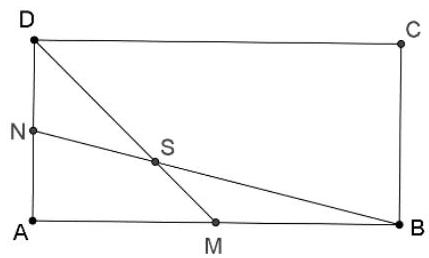
\includegraphics[max width=\textwidth, center]{2024_11_21_453869ede2e906b091c4g-1(1)}\\
\(20 a+19 b=365\). Znajdź wartości \(20 b+19 a\).
  \item Pijąc jedną szklankę czarnej herbaty zyskuje się kofeinę na 1 godzinę. Pijąc jedną szklankę kawy zyskuje się kofeinę na 4 godziny. W jakim stosunku należy wymieszać czarną herbatę i kawę, by uzyskać pełną szklankę zawierającą kofeinę na 2 godziny?
\end{enumerate}

\section*{KLASY PO GIMNAZJUM}
\begin{enumerate}
  \item Wyznacz wszystkie pary \((x, y)\) dodatnich liczb całkowitych spełniające równanie
\end{enumerate}

\[
(x+y)+(x-y)+x y+\frac{x}{y}=2020
\]

\begin{enumerate}
  \setcounter{enumi}{1}
  \item Marysia miała 11 jednakowych zapałek. Z dziewięciu ułożyła trójkąt o bokach: „2", ,„3", „4". Chciałaby za pomocą dwóch pozostałych zapałek podzielić ten trójkąt na dwie figury o równych polach. Czy jest to możliwe? Jeśli tak, pokaż sposób podziału. Uwaga: zapałek nie łamiemy, ani nie nakładamy na siebie.
  \item Danych jest pięć stycznych okręgów jak pokazano na rysunku. Znajdź promień najmniejszego okręgu, jeśli promień największego okręgu wynosi 2 , natomiast promienie dwóch okręgów z zaznaczonymi środkami są równe.\\
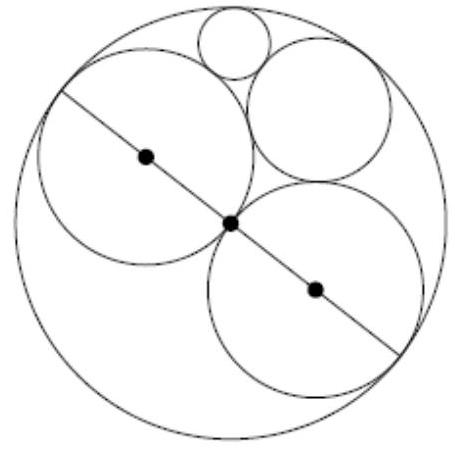
\includegraphics[max width=\textwidth, center]{2024_11_21_453869ede2e906b091c4g-1}
\end{enumerate}

\end{document}